\let\negmedspace\undefined
\let\negthickspace\undefined
\documentclass[journal]{IEEEtran}
\usepackage[a5paper, margin=10mm, onecolumn]{geometry}
%\usepackage{lmodern} % Ensure lmodern is loaded for pdflatex
\usepackage{tfrupee} % Include tfrupee package

\setlength{\headheight}{1cm} % Set the height of the header box
\setlength{\headsep}{0mm}     % Set the distance between the header box and the top of the text

\usepackage{gvv-book}
\usepackage{gvv}
\usepackage{cite}
\usepackage{amsmath,amssymb,amsfonts,amsthm}
\usepackage{algorithmic}
\usepackage{graphicx}
\usepackage{textcomp}
\usepackage{xcolor}
\usepackage{txfonts}
\usepackage{listings}
\usepackage{enumitem}
\usepackage{mathtools}
\usepackage{gensymb}
\usepackage{comment}
\usepackage[breaklinks=true]{hyperref}
\usepackage{tkz-euclide} 
\usepackage{listings}
% \usepackage{gvv}                                        
\def\inputGnumericTable{}                                 
\usepackage[latin1]{inputenc}                                
\usepackage{color}                                            
\usepackage{array}                                            
\usepackage{longtable}                                       
\usepackage{calc}                                             
\usepackage{multirow}                                         
\usepackage{hhline}                                           
\usepackage{ifthen}                                           
\usepackage{lscape}
\usepackage{circuitikz}
\tikzstyle{block} = [rectangle, draw, fill=blue!20, 
    text width=4em, text centered, rounded corners, minimum height=3em]
\tikzstyle{sum} = [draw, fill=blue!10, circle, minimum size=1cm, node distance=1.5cm]
\tikzstyle{input} = [coordinate]
\tikzstyle{output} = [coordinate]


\begin{document}

\bibliographystyle{IEEEtran}
\vspace{3cm}

\title{2.4.41}
\author{EE25BTECH11044 - Sai Hasini Pappula}
 \maketitle
% \newpage
% \bigskip
{\let\newpage\relax\maketitle}

\renewcommand{\thefigure}{\theenumi}
\renewcommand{\thetable}{\theenumi}
\setlength{\intextsep}{10pt} % Space between text and floats


\numberwithin{equation}{enumi}
\numberwithin{figure}{enumi}
\renewcommand{\thetable}{\theenumi}

\textbf{Question:} \\
Determine whether the points 
$A(3,6,9)$, $B(10,20,30)$, $C(24,-41,5)$
are the vertices of a right-angled triangle using matrices.

\bigskip

\textbf{Solution:} \\

% Positions
\begin{equation}
\myvec{A}=\begin{bmatrix}3\\6\\9\end{bmatrix},\quad
\myvec{B}=\begin{bmatrix}10\\20\\30\end{bmatrix},\quad
\myvec{C}=\begin{bmatrix}24\\-41\\5\end{bmatrix}.
\tag{1}
\end{equation}

% Side (difference) vectors — no AB/BC/AC notation
\begin{equation}
\myvec{B}-\myvec{A}
=\begin{bmatrix}10-3\\20-6\\30-9\end{bmatrix}
=\begin{bmatrix}7\\14\\21\end{bmatrix},
\quad
\myvec{C}-\myvec{B}
=\begin{bmatrix}24-10\\-41-20\\5-30\end{bmatrix}
=\begin{bmatrix}14\\-61\\-25\end{bmatrix},
\quad
\myvec{C}-\myvec{A}
=\begin{bmatrix}24-3\\-41-6\\5-9\end{bmatrix}
=\begin{bmatrix}21\\-47\\-4\end{bmatrix}.
\tag{2}
\end{equation}

% Dot products (matrix form), expanded
\begin{equation}
(\myvec{B}-\myvec{A})^{\!T}(\myvec{C}-\myvec{A})
=
\begin{bmatrix}7&14&21\end{bmatrix}
\begin{bmatrix}21\\-47\\-4\end{bmatrix}
=
7\cdot21+14\cdot(-47)+21\cdot(-4)
=-595 \neq 0.
\tag{3}
\end{equation}

\begin{equation}
(\myvec{B}-\myvec{A})^{\!T}(\myvec{C}-\myvec{B})
=
\begin{bmatrix}7&14&21\end{bmatrix}
\begin{bmatrix}14\\-61\\-25\end{bmatrix}
=
7\cdot14+14\cdot(-61)+21\cdot(-25)
=-1281 \neq 0.
\tag{4}
\end{equation}

\begin{equation}
(\myvec{C}-\myvec{A})^{\!T}(\myvec{C}-\myvec{B})
=
\begin{bmatrix}21&-47&-4\end{bmatrix}
\begin{bmatrix}14\\-61\\-25\end{bmatrix}
=
21\cdot14+(-47)\cdot(-61)+(-4)\cdot(-25)
=3261 \neq 0.
\tag{5}
\end{equation}

Since none of the products is zero, no angle of the triangle is $90^\circ$.

\bigskip

\textbf{Conclusion:} \\
The points $A$, $B$, and $C$ do \textbf{not} form a right-angled triangle.
\begin{center}
    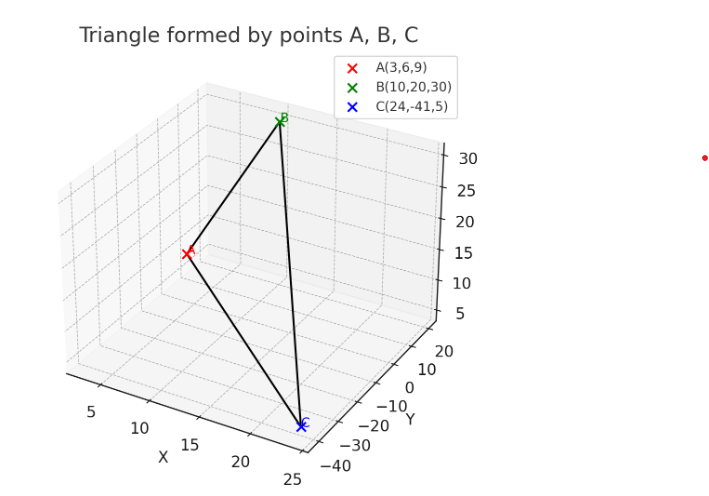
\includegraphics[width=0.8\columnwidth]{figs/plot3.png}
\end{center}

\end{document}


